%!TEX root = ../../../thesis.tex

Water metering is becoming increasingly common throughout the world~\cite{Chang2012}.
Sourcing and processing drinkable water is an expensive task.
As water rescources become constrained, volumetric charging, and therefore metering, become increasing important.
Cheap and reliable methods for reading meters will become more important as metering becomes prevalent.
Harvesting energy at the location of metering would eliminate the need for batteries.
Furthermore, removing the moving parts of traditional electrical generation devices should increase lifespan due to lower component wear.
This section investigates the feasibility of using streaming cell technology as a means of powering electronic water meters.

In \cref{chap:harvestingEnergy} we discussed electric power generation from streaming cells.
I demonstrated a \SI{0.2}{\micro\percent} conversion efficiency from water flow and pressure.
I showed that streaming voltage is directly proportional to the pressure across a cell.
Can that pressure dependence give a way to meter water consumption while generating power? Probably.
However, questions like this are only relevant if the harvester is feasible.
To find that out, the following questions must be answered:
\begin{enumerate}
  \item What quantity of energy is there available to harvest?
  \item What fraction can be harnessed?
  \item How much power do we need?
\end{enumerate}
The answer to the second question was answered in \cref{chap:harvestingEnergy}, (\SI{0.0002}{\percent}; and the answer to the third will be answered in the in \cref{chap:energyRequirements}.
This chapter addresses the amount of energy available to harvest in a typical domestic setting.


\section{Current Trends in Water Metering}
  Domestic and commercial water metering is becoming increasingly common throughout the world~\cite{Chang2012}.
  Water sourcing and processing is an expensive task for city councils.
  Cheap and reliable methods for retrieving metering information will become more important as water becomes more precious.

  In New Zealand - Auckland City, Tauranga City, Nelson City, Whangarei District and the Tasman District have already implemented water metering~\cite{WaterNewZealand2011}.
  For residents of Wellington, New Zealand's capitol city, water metering is optional.
  In metered locations, meter readers must manually read the display of each meter; a long and laborious task.
  
  Automatic meter reading systems (AMR) are an alternative method of collecting that data.
  Hamilton City Council is trialling such systems in remote areas in the hopes of adopting them for wide-spread use.
  There are two types of automatic meter reading systems:
  an external reader/transmitter that attaches to a compatible meter, or a meter built specifically for the purpose.

  Automatic meter reading systems offer advantages separate from making the meter-reader redundant.
  Increased billing frequency helps customers reduce their consumption by giving greater feedback.
  An automatic system removes the need to access a customers property~\cite{Chang2012}.
  Electronic analysis of the meters readings provides an easy way to detect water leaks.
  It is estimated that \SI{10}{\percent} of post-meter water consumption is due to leakage in the residential sector.
  Britton et al.\ show that communicating with customers whose homes showed signs of leakage that a night-time flow reduction of \SI{89}{\percent} is achievable.
  In contrast, a control group's night-time usage increased by over \SI{50}{\percent} in the same time-frame.
  Benefits of automatic water metering are not only geared toward billing, but improving the network as a whole.

  \begin{figure}
    \centering
    \includegraphics[width=0.9\textwidth]{content/pt1/02-WirelessWaterMeter/graphics/meter}
    \caption{\label{fig:Photo_DomesticWaterMeter}Photograph of a domestic water meter, and installation, (Kent PSMT 25mm) typical of an Auckland residential area.}
  \end{figure}

  Domestic water meters are typically installed at a property's boundary, in a plastic box set into the ground.
  An installation typical for an Auckland residential area is presented as~\cref{fig:Photo_DomesticWaterMeter}.
  The meter is installed over five eight meters into the property from the road-side.
  Because of its location, it is not feasible to connect it to a source of power.
  No commercially available domestic energy harvesting water meters, suitable for burial, exist on the market as of 2015.

  \begin{figure}
    \centering
    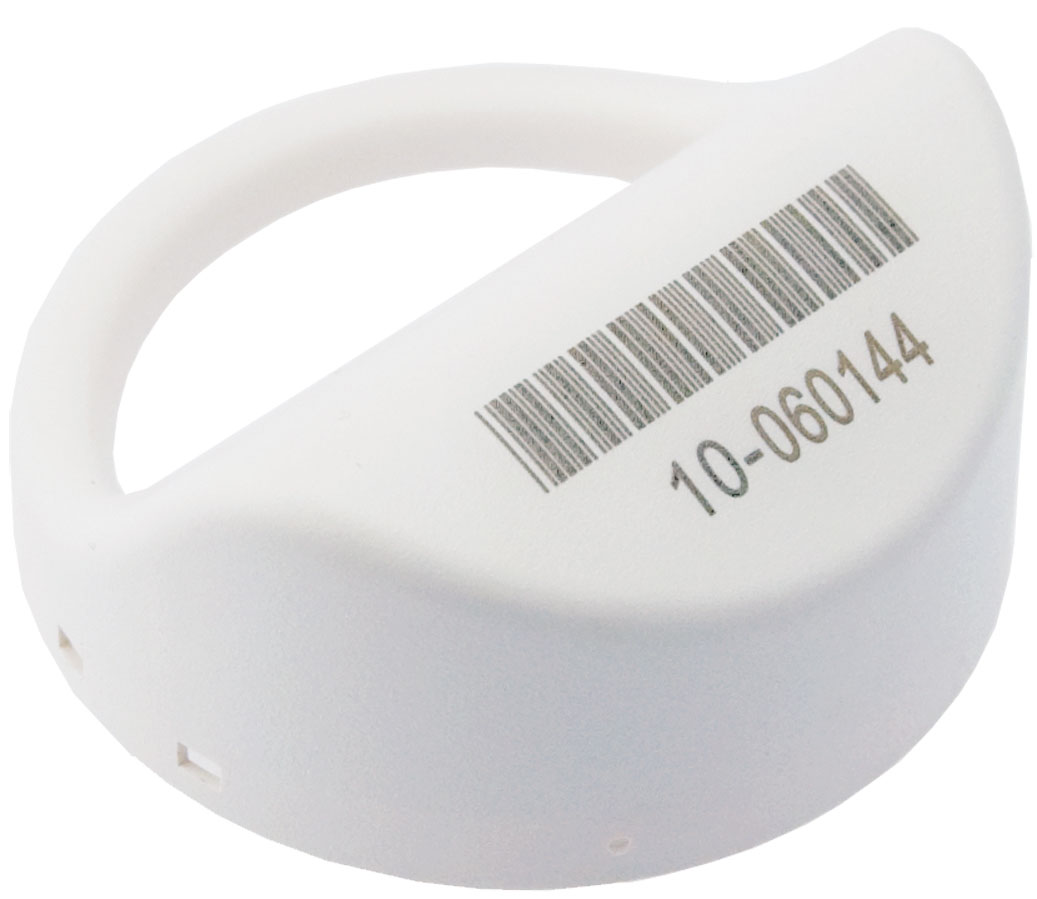
\includegraphics[width=0.5\textwidth]{content/pt1/02-WirelessWaterMeter/graphics/hydro-WMBUSWLESSM}
    \caption{
      \label{fig:Photo_waterwareMeter}
      Photograph of the a wireless transmitting module from Waterware NZ.
      The device attaches to a compatible water meter and contains its own battery~\cite{BMeters2014}.
    }
  \end{figure}

  A common configuration for wireless automatic meter reading is to have a reader/transmitter device that is separate to the meter itself.
  Such a device usually attaches to the meter's display or has a wire connecting it to the meter.
  Being detachable and tamper-proof means it must be powered by batteries.
  A commonly stated battery life for such units is ten years~\cite{BMeters2014}, close to batteries shelf-life.

  We investigate the possibility of replacing these batteries with a streaming cell based energy harvester.
  A harvester removes the need for batteries, but needs to be plumbed into the water feed.
  The resulting device would most likely replace the meter, as opposed to being an attachment. 

  \section{Envisioned harvester design}

    In \cref{chap:harvestingEnergy}, energy was converted between fluid-mechanical to electrical using a single channel.
    Harvesting for electronic water meters will require more energy than that channel could produce.
    There are multiple ways of scaling the streaming cell design used in \cref{chap:harvestingEnergy}.
    The channel can be made wider, doubling the width will double the output power;
    multiple channels can be stacked together, multiplying the output by the number of channels formed.
    Scaling the harvester is not considered a problem, but the pressure drop it develops is.
    High fluid resistance is inevitable since practical efficiencies are only obtained when the internal dimensions are small.

    \begin{figure}
      \centering
      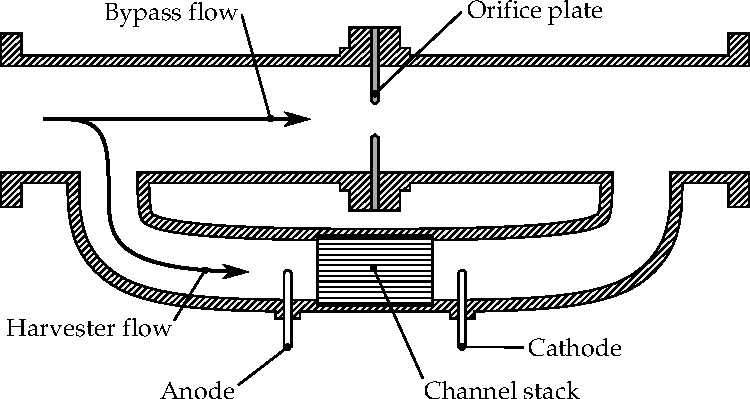
\includegraphics[width=0.9\textwidth]{content/pt1/02-WirelessWaterMeter/graphics/harvester}
      \caption{\label{fig:Diagram_harvester}Diagram showing the intended design of streaming cell harvester suitable for domestic connection.}
    \end{figure}

    To control the pressure drop across the harvester, the mechanical design shown in~\cref{fig:Diagram_harvester} is proposed.
    It gives the capability of controlling the hydrodynamic resistance of the unit as a whole by means an orifice plate.
    The plate sits in the ``main line'' causing a pressure differential in proportion to the flow rate.
    An orifice plate with a hole equal in diameter to the main pipe causes no pressure differential as it causes no flow obstruction.
    Conversely, a plate without a hole forces all liquid through the harvester, causing the maximum pressure differential.
    Using an appropriate sized orifice plate, the customer will be unaware of the harvester's presence and a suitable pressure differential will be developed.
    
    For the sake of analysis we assume the orifice plate will be sized to match the pressure loss of a mechanical meter.
    This assumption means the amount of harvestable energy is equal to the amount dissipated in a mechanical water meter.
    The following section quantifies the amount of energy a water meter dissipates over an average week in a typical Auckland home.


  \section{Quantifying harvestable energy} 

    This section estimates the quantity of energy available to a harvester placed in a domestic feed.
    Using a bypass pipe with an orifice plate the pressure drop across the harvester can be controlled.
    This means the pressure drop across the harvester can be set to match that of a mechanical meter.
    The amount of harvestable energy under this assumption is the amount of energy dissipated inside a mechanical meter.

    \begin{table}
      \centering
      \begin{tabular}{r l|r|r|l}
        Item                    & Measurement & Summer & Winter & Unit\\
        \hline\hline
        \multirow{4}{*}{Shower} & Duration    & 6.6    & 7.0    & minutes\\
                                & Volume      & 50.0   & 52.5   & litres\\
                                & Flow        & 8.1    & 8.0    & litres/minute\\
                                & Frequency   & 0.9    & 0.9    & /person/day\\
        \hline
        \multirow{2}{*}{Washing}& Volume      & 122    & 123    & litres\\
                                & Frequency   & 0.35   & 0.36   & /person/day\\
        \hline
        \multirow{2}{*}{Toilet} & Volume      & 6.6    & 6.8    & litres\\
                                & Frequency   & 4.9    & 4.5    & /person/day\\
      \end{tabular}
      \caption{
          \label{tab:consumption_figures}
          Average usage characteristics for a shower, washing machine and toilet.
          Data obtained from~\cite{Heinrich2008}.
      }
    \end{table}

    In 2008, Heinrich monitors water consumption of 51 homes throughout Auckland in 2008~\cite{Heinrich2008}.
    The report shows that the majority of domestic water is consumed by the shower (\SI{30}{\percent}), washing machine (\SI{27}{\percent}) and toilet (\SI{20}{\percent}).
    Together these account for over \SI{75}{\percent} of domestic water consumption.
    Data from \cref{tab:consumption_figures} was used to build a typical water usage profile.
    Heinrich published a similar report in 2007 that contained water flow profiles, the flow profile of the toilet has been taken from that report~\cite{Heinrich2007}.
    
    \begin{figure}
      \centering
      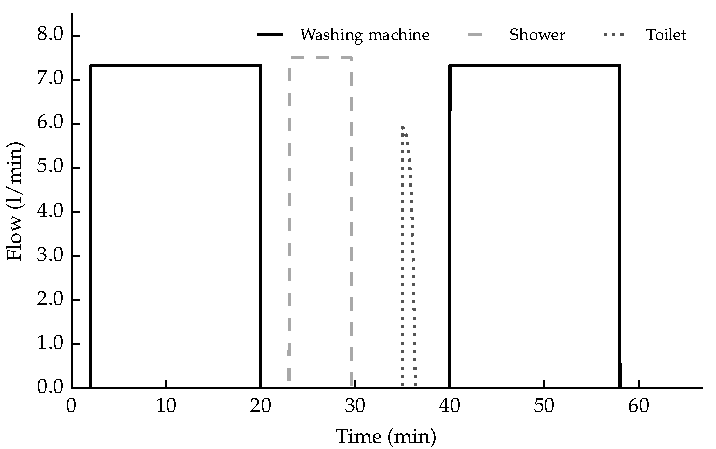
\includegraphics[width=\linewidth]{content/pt1/02-WirelessWaterMeter/graphics/graph_profile}
      \caption{
          Sample profile showing constructed instances of washing machine use, a shower and a toilet flush.
          The washing machine's wash and rinse cycles are separated in time.}
      \label{fig:profileSample}
    \end{figure}

    \Cref{fig:profileSample} shows the flow rates for each of the three items considered (toilet, shower and washing machine).
    Volumes for each of the events, and flow profile of the toilet, match data given by Heinrich.
    Specifically the total volumes for each are: \SI{122}{\litre}, \SI{49.5}{\litre} and \SI{6.22}{\litre} for the washing machine, shower and toilet respectively.

    \begin{figure}
        \centering
        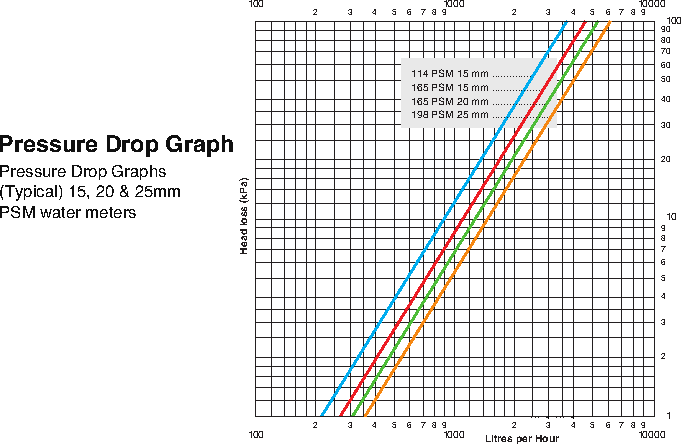
\includegraphics[width=\linewidth]{content/pt1/02-WirelessWaterMeter/graphics/Kent-PSM-HeadLoss}
        \caption{
            \label{fig:headloss}
            Log-log graph showing the pressure developed across the Kent PSM series mechanical water meters. Taken from~\cite{Elster2008}.
        }
    \end{figure}

    The Kent 25-PSMT series mechanical water meter is the most commonly used water meter in the Auckland district~\cite{WatercareNewZealand2014}.
    \Cref{fig:headloss} shows the head loss versus flow rate for the Kent PSM range of meters.
    The following equation fits the trace for the \SI{25}{\milli\meter} PSMT meter:
    \begin{equation}
        \Delta P = e^{3.725\thinspace log(flow) - 9.5}
        \label{eqn:Flow_to_pressure_25mmPSMT}
    \end{equation}

    \begin{figure}
        \centering
        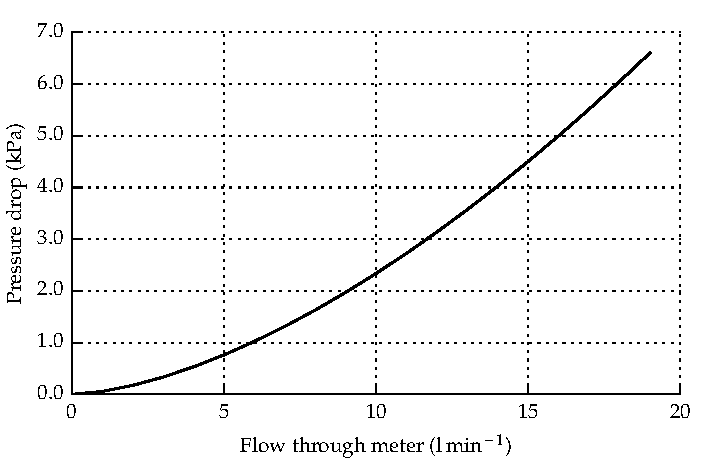
\includegraphics[width=\linewidth]{content/pt1/02-WirelessWaterMeter/graphics/graph_pressureLoss}
        \caption{Graph showing fitted curve to the pressure loss graph presented as \cref{fig:headloss}.}
        \label{fig:headloss_fit}
    \end{figure}

    \Cref{eqn:Flow_to_pressure_25mmPSMT} is plotted in \cref{fig:headloss_fit} on linear scales.

    The profile fits the usage statistics of a home with two occupants according to the previously mentioned reports over the duration of a week.
    During that time five uses of a washing machine, fourteen showers and fifty six toilet flushes occur.
    \Cref{fig:profileSample} shows
    A sample of the usage profiles of each item is shown in Fig. \ref{fig:profileSample}.

    \begin{figure}
        \centering
        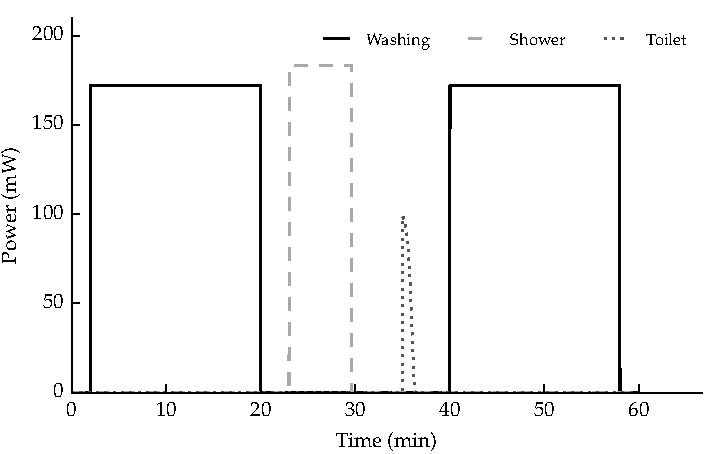
\includegraphics[width=\linewidth]{content/pt1/02-WirelessWaterMeter/graphics/graph_harvest}
        \caption{Calculated power dissipation by a typical domestic mechanical water meter for each of the sample profile events.}
        \label{fig:powerDissipated_meter}
    \end{figure}

    Fig.~\ref{fig:headloss} shows the pressure head loss curve from a water meter typically installed at New Zealand homes (Kent PSMT 25mm)~\cite{WatercareNewZealand2014}.

    Using this curve we calculate power dissipation in a water meter during a washing machine cycle, shower, and toilet flush; presented as \cref{fig:powerDissipated_meter}.
    The total energy dissipated within the meter for each events is:
    \begin{itemize}
    \item \SI{547}{\joule} per load of washing,
    \item \SI{222}{\joule} per shower, and
    \item \SI{24.3}{\joule} per flush of the toilet.
    \end{itemize}

% washing machine volume = 122.00 l
% shower volume = 49.50 l
% toilet volume = 6.22 l
% washing machine energy = 172.08 l
% shower energy = 72.62 l
% toilet energy = 5.07 l

    % These figures are based on average duration and flow rates as found in \cite{Heinrich2008}, and the estimated head loss from Fig.~\ref{fig:headloss}.
    Over an average week the reference water meter would dissipate approximately \SI{7.20}{\kilo\joule} of energy; averaging \SI{1.03}{\kilo\joule} per day.


